

\tikzset{every picture/.style={line width=0.75pt}} %set default line width to 0.75pt        

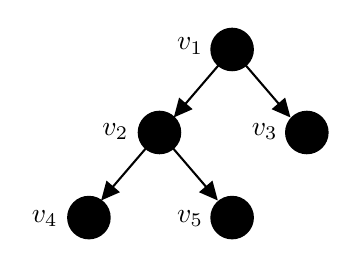
\begin{tikzpicture}[x=0.75pt,y=0.75pt,yscale=-1,xscale=1]
%uncomment if require: \path (0,151); %set diagram left start at 0, and has height of 151

%Straight Lines [id:da6269794272523825] 
\draw    (95,70) -- (121.15,100.47) ;
\draw [shift={(123.1,102.75)}, rotate = 229.37] [fill={rgb, 255:red, 0; green, 0; blue, 0 }  ][line width=0.08]  [draw opacity=0] (8.93,-4.29) -- (0,0) -- (8.93,4.29) -- cycle    ;
%Straight Lines [id:da986476888481959] 
\draw    (130,30) -- (156.15,60.47) ;
\draw [shift={(158.1,62.75)}, rotate = 229.37] [fill={rgb, 255:red, 0; green, 0; blue, 0 }  ][line width=0.08]  [draw opacity=0] (8.93,-4.29) -- (0,0) -- (8.93,4.29) -- cycle    ;
%Straight Lines [id:da44376792645731866] 
\draw    (95,70) -- (68.85,100.47) ;
\draw [shift={(66.9,102.75)}, rotate = 310.63] [fill={rgb, 255:red, 0; green, 0; blue, 0 }  ][line width=0.08]  [draw opacity=0] (8.93,-4.29) -- (0,0) -- (8.93,4.29) -- cycle    ;
%Straight Lines [id:da9694685289799305] 
\draw    (130,30) -- (103.85,60.47) ;
\draw [shift={(101.9,62.75)}, rotate = 310.63] [fill={rgb, 255:red, 0; green, 0; blue, 0 }  ][line width=0.08]  [draw opacity=0] (8.93,-4.29) -- (0,0) -- (8.93,4.29) -- cycle    ;
%Shape: Circle [id:dp9985907627673265] 
\draw  [fill={rgb, 255:red, 0; green, 0; blue, 0 }  ,fill opacity=1 ] (120,30) .. controls (120,24.48) and (124.48,20) .. (130,20) .. controls (135.52,20) and (140,24.48) .. (140,30) .. controls (140,35.52) and (135.52,40) .. (130,40) .. controls (124.48,40) and (120,35.52) .. (120,30) -- cycle ;
%Shape: Circle [id:dp9359075911835515] 
\draw  [fill={rgb, 255:red, 0; green, 0; blue, 0 }  ,fill opacity=1 ] (156,70) .. controls (156,64.48) and (160.48,60) .. (166,60) .. controls (171.52,60) and (176,64.48) .. (176,70) .. controls (176,75.52) and (171.52,80) .. (166,80) .. controls (160.48,80) and (156,75.52) .. (156,70) -- cycle ;
%Shape: Circle [id:dp3437213039907303] 
\draw  [fill={rgb, 255:red, 0; green, 0; blue, 0 }  ,fill opacity=1 ] (85,70) .. controls (85,64.48) and (89.48,60) .. (95,60) .. controls (100.52,60) and (105,64.48) .. (105,70) .. controls (105,75.52) and (100.52,80) .. (95,80) .. controls (89.48,80) and (85,75.52) .. (85,70) -- cycle ;
%Shape: Circle [id:dp8935393527337947] 
\draw  [fill={rgb, 255:red, 0; green, 0; blue, 0 }  ,fill opacity=1 ] (51,111) .. controls (51,105.48) and (55.48,101) .. (61,101) .. controls (66.52,101) and (71,105.48) .. (71,111) .. controls (71,116.52) and (66.52,121) .. (61,121) .. controls (55.48,121) and (51,116.52) .. (51,111) -- cycle ;
%Shape: Circle [id:dp3004114626227925] 
\draw  [fill={rgb, 255:red, 0; green, 0; blue, 0 }  ,fill opacity=1 ] (120,111) .. controls (120,105.48) and (124.48,101) .. (130,101) .. controls (135.52,101) and (140,105.48) .. (140,111) .. controls (140,116.52) and (135.52,121) .. (130,121) .. controls (124.48,121) and (120,116.52) .. (120,111) -- cycle ;

% Text Node
\draw (102,23) node [anchor=north west][inner sep=0.75pt]    {$v_{1}$};
% Text Node
\draw (66,64) node [anchor=north west][inner sep=0.75pt]    {$v_{2}$};
% Text Node
\draw (138,64) node [anchor=north west][inner sep=0.75pt]    {$v_{3}$};
% Text Node
\draw (102,106) node [anchor=north west][inner sep=0.75pt]    {$v_{5}$};
% Text Node
\draw (32,106) node [anchor=north west][inner sep=0.75pt]    {$v_{4}$};


\end{tikzpicture}